\documentclass[12pt,a4paper,english,twoside,openright]{report}
\usepackage{parskip}

\usepackage[includeheadfoot, inner=3.5cm, outer=3.5cm]{geometry}
\setlength{\headheight}{15pt}

\usepackage{emptypage}
\usepackage{pdfpages}

\usepackage{fancyhdr}
\pagestyle{fancy}
\fancyhf{}
\fancyhead[LE,RO]{\thepage}
\renewcommand{\sectionmark}[1]{ \markright{\thesection\ #1}{} }
\fancyhead[RE,LO]{\rightmark}

\usepackage{float}
\floatstyle{boxed}
\restylefloat{figure}

\usepackage[
  colorinlistoftodos,
  prependcaption,
  textsize=small
]{todonotes}

\usepackage[utf8]{inputenc}
\usepackage[T1]{fontenc,url}
\urlstyle{sf}

\usepackage{amssymb}
\usepackage{tikz}
\usetikzlibrary{matrix,arrows,backgrounds,fit}

\usepackage{minted}
\newmintinline[ir]{rust}{}
\newmintedfile[rustfile]{rust}{}

\usepackage{babel,textcomp,csquotes,varioref,graphicx}

\usepackage[
  backend=biber,
  maxbibnames=6,
  isbn=false,
  doi=false,
  defernumbers=true
]{biblatex}
\addbibresource{refs.bib}
\setlength\bibitemsep{\baselineskip}

\usepackage[
  pdftitle={Efficient Persistent Vector Implementation for Rust},
  pdfauthor={Araz Abishov},
  hidelinks=true,
  unicode=true  
]{hyperref}
\urlstyle{same}

\newcommand{\bigo}[1] { $\mathcal{O}(#1)$ }

\newcommand{\rbtree} { RB-Tree }
\newcommand{\m} { $m$ }
\newcommand{\h} { $h$ }
\newcommand{\x} { $x$ }

\colorlet{color-path}{blue!30}
\colorlet{color-node}{blue!10}

\title{Efficient Persistent Vector Implementation for Rust}
\author{Araz Abishov}

\begin{document}

\pagenumbering{roman}
\includepdf[pages={-}]{forside/forside.pdf}
\setcounter{page}{5}

\pdfbookmark[0]{Front matter}{bm-frontmatter}
\pdfbookmark[1]{Contents}{bm-toc}
\tableofcontents{}

\cleardoublepage
\pdfbookmark[1]{List of Listings}{bm-listings}
\listoflistings

\cleardoublepage
\pdfbookmark[1]{List of Figures}{bm-figures}
\listoffigures

\cleardoublepage
\vspace*{2cm}
\thispagestyle{plain}

\phantomsection
\addcontentsline{toc}{section}{Abstract}

\begin{center}
\section*{Abstract}
\end{center}

Rust is a multi-paradigm system programming language focused on performance and reliability. Its rich type system guarantees memory and thread-safety at compile-time.

Rust forbids simultaneous sharing and mutation, that sometimes is a necessary and a useful pattern. A common way to mitigate this limitation in Rust is to clone a value before sharing it. Naive cloning by copying, however, is an expensive operation both in terms of memory and performance.

This thesis presents \pvecrs{}, a project that contributes a vector implementation with efficient clone operation that borrows ideas from persistent data structures. The project explores novel approaches to optimize vector’s performance by leveraging type system of Rust, as well as aiming to achieve convenient, idiomatic interface familiar to developers. The proposed optimizations are evaluated and discussed based on results of the sequential and parallel tests.


\cleardoublepage
\vspace*{2cm}
\thispagestyle{plain}

\begin{center}

\phantomsection
\addcontentsline{toc}{section}{Acknowledgements}

\section*{Acknowledgements}

\end{center}

I would like to thank my supervisors, Martin Steffen and Volker Stolz, for their guidance and feedback. Without their patience and support, as well as trust in my own idea, this venture would not have been possible.

My deepest appreciation goes to my family and my friends for their moral support, their continuous encouragement, and their help whenever it was needed.

Finally, I would like to thank the Rust community for being so welcoming and supportive. In particular, I am grateful to Nicholas D. Matsakis for inspiring me to work on this project.


\cleardoublepage
\thispagestyle{plain}

\begin{center}
    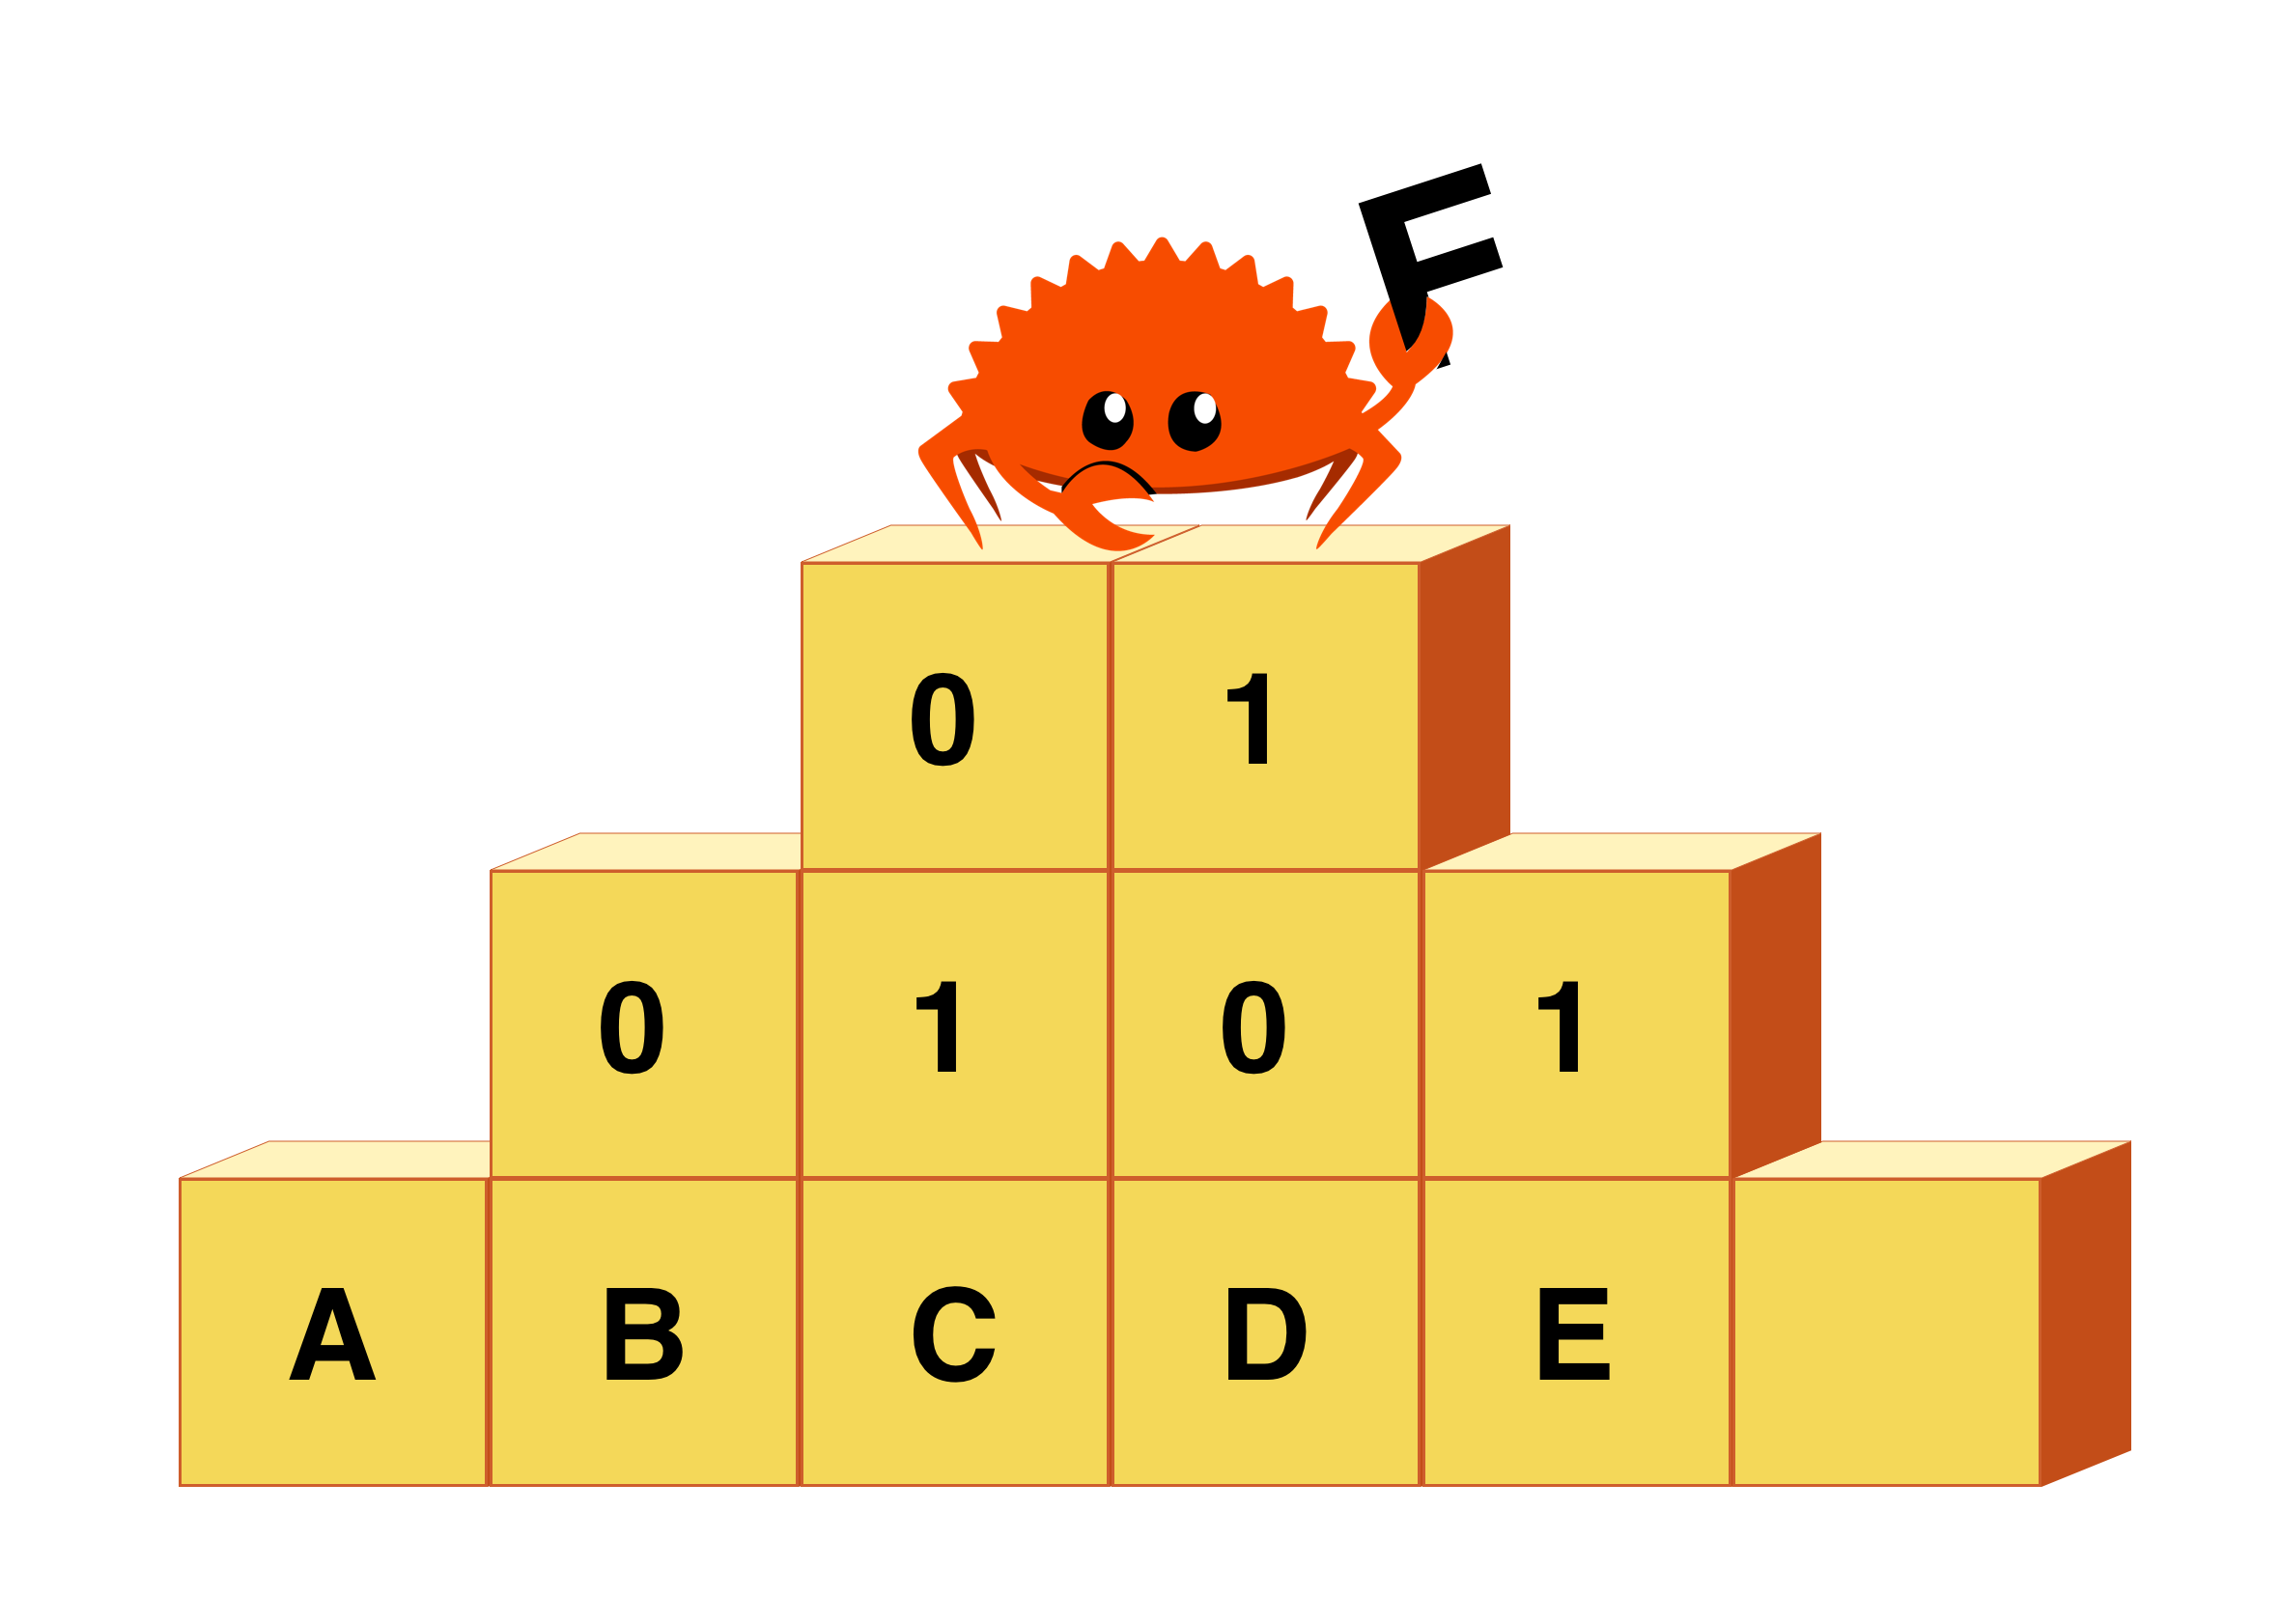
\includegraphics[width=8cm, angle=0, trim=10 10 10 10, clip]{images/ferris-climbing.png}

    \phantomsection
    \addcontentsline{toc}{section}{Reading notes}

    \section*{Reading notes}
    \begin{justify}
        The links to the LaTeX source code and the latest version of this document can be found at \url{https://abishov.com/thesis/}. The implementation, documentation, and visualization demo can be found at \url{https://abishov.com/pvec-rs}.

        If you notice any typos while reading the document, or have any feedback in general, feel free to open an issue at \url{https://github.com/arazabishov/thesis/issues} or send me an email at \href{mailto:araz@abishov.com}{\nolinkurl{araz@abishov.com}}.

        \paragraph{Colophon}
        The illustration above with Ferris\footnote{Unofficial mascot for Rust: \url{https://rustacean.net/}} sitting on top of \treerrb{}, kindly prepared by Vanessa Tesorone. The reading notes design and the idea to use Rust's mascot for the document decoration was inspired by the master's thesis of Erik Vesteraas\footnote{\url{http://erik.vestera.as/thesis/}}.
    \end{justify}

    \subsection*{Typographic conventions}
    \begin{tabular}{ r l }
        Clickable link & \href{https://www.rust-lang.org/}{Rust Programming Language} \\
        Inline code and types & \mintinline{rust}{Vec::new()} \\
        Project or library name & \pvecrs{} \\
    \end{tabular}

\end{center}


\pagenumbering{arabic}

\chapter{Introduction}

% TODO: Optional<Add a point to introduction to describe what is RefCell>
% TODO: Linear types (from Jean's work):
% Earlier work has lead to the definition of linear types, a way to define mutable types in a similar fashion as transients, with focus on correctness [20]. A linear type can only be used once, although relaxed constraints provide means to temporarily define a linear type as nonlinear, which gives users read capabilities without “using” the instance. In contrast, a transient is an affine type, where the function persistent! converts the affine nodes permanently to nonlinear, persistent nodes. 
% TODO: Linear types can change the world

\section{Persistent data structures}

A vast majority of modern programming languages are equipped with a standard library --- a set of constructs and utilities aimed to improve the developer's productivity. 

A significant part of standard library consists of commonly used data structures such as lists, sets, and maps, which often provide operations for reading and writing data. 

Modifying or \emph{mutating} an \emph{ephemeral} data structure implies that we no longer will have access to its older version. In contrast, a \emph{persistent} data structure allows access to any version, old or new, at any time \cite{making-data-structures-persistent}. 

Persistent data structures could be classified based on the operations which they offer over their versions:
\begin{itemize}
    \item \textit{Partial persistence} --- In this persistence model, we can query any previous version of the data structure, but we can update only the newest version. The versions are linearly ordered. 
    \item \textit{Full persistence} --- Both access and updates are allowed on all versions. The versions can be visualized as a branching tree.
    \item \textit{Confluent persistence} --- In addition to the previous operations, it offers combination operation to merge more than one previous version to output a new single version. The versions form a directed acyclic graph \cite{fully-persistent-lists-with-catenation}.  
    \item \textit{Functional persistence} --- This model takes its name from functional programming where objects are immutable. In comparison to the previous models, it prohibits change of the internal representation of the data structure \cite{purely-functional-data-structures}. 
\end{itemize}

While persistence can be achieved by simple copying, the performance of a modification operation quickly becomes unacceptable. This led to research and development of more efficient solutions, which were often designed to solve particular problems. A lack of general purpose collections, which guarantee uniformly good performance across different operations, results in challenges with software development. 

A persistent \emph{vector}, also known as a one-dimensional growable array, is very inefficient if implemented naively. Each update operation will cause a full copy of the underlying array, consuming additional amount of memory and processor time. 

However most operations modify only some parts of data structures, a complete copy is redundant. A better approach is to exploit the similarity between the new and old versions by \emph{sharing} structure between them. For example, instead of representing a data structure as a single block of memory, it could be broken down into smaller pieces or \emph{nodes}, which are linked together in the form of a \emph{tree}. Since modifications only apply to some nodes, the rest of them still remain unchanged and can be shared without copying. 

The first persistent vector implementation which offered good performance across a broad range of operations was introduced by Rich Hickey in the Clojure programming language. It was based on Phil Bagwell's Hash Array Mapped Trie \cite{ideal-hash-trees}, which offers practically constant runtime for push, update, and access operations, and it is a \emph{fully} persistent data structure. 

Later Phill Bagwell introduced a confluently persistent vector based on Relaxed Radix Balanced Tree \cite{efficient-immutable-vectors}, which has improved performance of the concatenation operation significantly and became a foundation for Scala's standard library vector implementation. 

The project presented in the thesis contributes an efficient persistent vector implementation for Rust based on Relaxed Radix Balanced Tree, which takes advantage of the Rust's type system to improve performance, guarantee thread safety and provide an idiomatic application programming interface. In order to ensure the best possible average performance, its internal representation switches from standard vector to RRB-Tree during runtime. 

\section{The Rust programming language}
\todo{The Rust programming language}

\subsection{Ownership and borrowing}
\todo{Ownership and borrowing}

\subsection{Reference counting and memory management}
\todo{Reference counting and memory management}

\section{Contributions}
\todo{Contributions}

\chapter{Radix Balanced Tree}

Radix Balanced Tree or \emph{\rbtree}, is a tree like data structure where each node has at most \m{} number of children and uses element indices as keys. It was first introduced by Rich Hickey as a basis for the persistent vector implementation in the Clojure's standard library \cite{the-clojure-programming-language}. 

Most data structures are tailored to specific use cases, with some operations being faster than others. For example, a persistent linked list can prepend elements and read the head in \bigo{1} time. However, random access is proportional to \bigo{n}, which is unacceptable in practical scenarios. 

In comparison, the Clojure's vector implementation is delivering \emph{practically} \bigo{1} time on fundamental operations such as access, update, push, and pop, rivaling ephemeral vector in performance.

This chapter introduces the inner workings of \rbtree{} and covers algorithms used in core operations. For more formal description of the persistent vector refer to \cite{improving-performance-through-transience}. 

\section{Memory layout}
\label{sec:rb-tree-memory-layout}

\rbtree{} consists of nodes which contain references either to other sub-trees or values. We will be calling the former type of node as \emph{branch} node, while the latter one as \emph{leaf}. The number of sub-trees and values in the node is configurable and will be denoted as \m{}, also known as \emph{branching factor}. 

When \m{} is set to a large value, \rbtree{} becomes wide and shallow. In practice, the branching factor is set to 32 to achieve \emph{practically} \bigo{1} performance across different operations, but technically this number can be any power of 2.

From now and onwards the height of the tree will be referred to as \h{}. The upper bound of \h{} can be calculated using ${\log_m(n - 1) + 1}$, where $n$ is the total count of elements in the tree. If \m{} is 32 and the number of elements will never be larger than the maximum index representable with 32 bit signed integers, the maximum height of the tree won't exceed 7 levels. 

References to values are stored at the leaf nodes of the tree. If the count of values stored in the structure is less than branching factor, then the root node itself will be a leaf. Otherwise, capacity of the tree is increased by adding intermediate, branch nodes, which contain references to other branches or leaves. 

\section{Radix search}

Before trying to understand how primitive operations such as push, pop and update work, let's take a look at how to access the right element in \rbtree{}. The lookup mechanism is called \emph{radix search}, a fundamental operation which forms the basis for other primitives.

Conceptually, the idea behind search in a tree-like structure boils down to picking correct nodes based on the given key. If there is a value corresponding to the key, we stop searching and return the value. Otherwise, an empty value or error is returned.

The lookup mechanism often depends on organization of nodes in the tree. Let's consider an example where each node can have at most two child nodes, called \emph{binary tree}. A binary tree where every node fits a specific ordering property is called \emph{binary search tree}. While searching, the key at each node is compared to the search key. All that is important is whether the key in the node is less than, equal to, or greater than the search key. The search is continued until an exact match or reaching leaf nodes.

Another tree-like data structure --- trie, also known as prefix tree, is interesting because its nodes do not store complete keys. Instead, each node stores only part of it. A trie is a variant of an n-ary tree in which characters are stored at each node. Each path down the tree may represent a word. A node in a trie could have anywhere from 0 through the size of the alphabet children. For example, English alphabet has 26 letters, meaning that each node in a trie might have up to 26 children.

The lookup procedure for tries involves breaking down the search key into multiple sub-keys, which are used to pick corresponding sub-tries. For example, the key "car" will be broken down into several smaller keys such as "c", "a", "r". If there is a value present at the last node of the path, it is returned. Otherwise, the search key is not present in the structure.

\subsection*{Bit partitioning}

\rbtree{} is a variation of a trie, which is also known as \emph{persistent bit-partitioned vector trie}. So what does make it so special? 

A search key in \rbtree{} is an integer, which can be viewed as a composite key, where each sub-key is represented by a sequence of bits. The idea is to divide the key into blocks of bits, where each block forms an index specific to the tree node. The count of bits in each of those chunks can be derived from the branching factor and will be called as \emph{bits per level}.

The \emph{bits per level} or \x{} is the count of bits used to address \m{} nodes in the binary numeral system. The relationship between \m{} and \x{} can be represented as: 

\begin{equation}
    2^x = m
\end{equation}

This leads us to a formula which derives the count of \emph{bits per level} from \m{}: 

\begin{equation}
    \label{eq:bits-per-level}
    x = log_2(m)
\end{equation}

For example, with \m{} equal to 16, the maximum index value is 15. 15 converted to the binary form is $1111_2$, which evidently requires 4 bits of space. If we substitute \m{} into \Cref{eq:bits-per-level}, we will get the same value. 

\subsection*{Extracting sub-keys}

Now when the size of the sub-key is known, next step is to identify its location. The count of sub-keys within the search key depends on the heght of the tree. Each new level in \rbtree{} will use \x{} additional bits of space. For instance, a search key addressing an element of the tree of ${h = 3}$ and ${x = 2}$ will consist of 3 sub-keys taking up 6 bits of space in total.

Sub-keys are arranged in the order from the most to the least significant bits, where the most significant sequence is a key used to access child node of the root. Each following key is used to index into child node on the corresponding tree level.

Knowing the depth at which a node is located and the count of bits per level, the value of the key can be calculated using bitwise operations such as logical shift and masking. Let's take a look at mechanism used to extract the right sub-key. 

In the following example there is a byte which represents a key equal to 54. Let's assume that it belongs to the tree where \m{} is 4, \x{} is 2 and that height of the tree 3. 

\begin{equation}
    54_{10} = 00110110_2    
\end{equation}

Since there are three levels, we have only three sub-keys: $11_2$, $01_2$ and $10_2$. Let's say that we are interested in extracting sub-key for the child node on the second level --- $01_2$. 

First, let's get rid of the bits following the sub-key of our interest. Logical right shift operation --- $\ggg$, will push $(l - 1) * x$ 0s into key, where $l$ is the \emph{level} at which current node is located. 

\begin{equation}
    00110110 \ggg ((l - 1) * x)
\end{equation}

Since the node in the example is located at $l = 2$ and $x = 2$, the search key will be shifted by 2. The result of operation is $00001101_2$. As you can see, the "tail" of the key is truncated.

The next step is to get rid of bits preceding the sub-key by masking them to 0. An operator used for this is known as bitwise "and" and it will be applied to the result of shifting operation. 

A bitwise "and" takes two equal-length binary representations and performs the logical "and" operation on each pair of the corresponding bits. 

Thus, if both bits in the compared position are 1, the bit in the resulting binary representation is 1; otherwise, the result is 0. Here is an example:

\begin{equation}
    00001101 \ \& \ 00000011 = 00000001
\end{equation}
                                    
The first and the second operands are the key and mask respectively. 

Only the last two bits of the mask are set to 1, which means that all bits of the key except last two will be masked to 0. The result of the "and"-ing operation will be the value of the sub-key.

Now the question is how to define a mask and what are the requirements to it. First of all, it has to be of the same type as the key, meaning that it must have the same count of bits in the binary representation. Secondly, the last \x bits must be set to 1.

The mask is equal to the maximum value of the sub-key, which can be calculated from the branching factor:

\begin{equation}
    mask = m - 1
\end{equation}

If \m{} is equal to 4 the maximum sub-key value will be 3, which equals to 00000011 in the binary representation.

\subsection*{Summary}

\begin{figure}        
    \caption{Accessing element at index 104 in a tree of height 4. Empty nodes represent collapsed subtrees.}
    \label{fig:rb-tree-example-1}

    \centering
    \begin{tikzpicture} [    
        node/.style = { 
            matrix of nodes, 
            nodes = { draw, minimum width = 6mm, minimum height = 8mm, anchor = center},
            font = \small,
            nodes in empty cells        
        },    
        value/.style = { 
            matrix of nodes, 
            nodes = { draw = none, minimum width = 4mm, minimum height = 4mm, anchor = center, rotate = 90 },
            font = \small,            
            nodes in empty cells        
        },    
        edge/.style = { ->, shorten >= 4pt }
    ]   
        \node[] (index) at (current page.north west) { $104_{10}$ = $01 10 10 00_{2}$ };        
        
        \matrix[node] (node-1-1) [below right = 8mm and 1cm of index] { 00 & 01 & 10 & 11 \\ };
                
        \scoped[on background layer] {
            \node[fit=(node-1-1-1-1), fill=color-node, inner sep = 0pt]   {};
            \node[fit=(node-1-1-1-2), fill=color-path, inner sep = 0pt]   {};
            \node[fit=(node-1-1-1-3), fill=color-node, inner sep = 0pt]   {};
            \node[fit=(node-1-1-1-4), fill=color-node, inner sep = 0pt]   {};
        }
        
        \matrix[node, inner sep = 0pt] (node-2-2) [below left = 8mm and 1mm of node-1-1.south] { 00 & 01 & 10 & 11 \\ };
        \matrix[node, fill = color-node, inner sep = 0pt] (node-2-3) [below right = 8mm and 1mm of node-1-1.south] { & & & \\ };
        \matrix[node, fill = color-node, inner sep = 0pt] (node-2-1) [left = 2mm of node-2-2.west] { & & & \\ };
        \matrix[node, fill = color-node, inner sep = 0pt] (node-2-4) [right = 2mm of node-2-3.east] { & & & \\ };

        \scoped[on background layer] {
            \node[fit=(node-2-2-1-1), fill=color-node, inner sep = 0pt]   {};
            \node[fit=(node-2-2-1-2), fill=color-node, inner sep = 0pt]   {};
            \node[fit=(node-2-2-1-3), fill=color-path, inner sep = 0pt]   {};
            \node[fit=(node-2-2-1-4), fill=color-node, inner sep = 0pt]   {};
        }

        \draw[edge, out=225, in=45] (node-1-1-1-1.south) to (node-2-1.north);
        \draw[edge, out=225, in=45] (node-1-1-1-2.south) to (node-2-2.north);
        \draw[edge, out=315, in=135] (node-1-1-1-3.south) to (node-2-3.north);
        \draw[edge, out=315, in=135] (node-1-1-1-4.south) to (node-2-4.north);

        \matrix[node, fill = color-node, inner sep = 0pt] (node-3-2) [below left = 8mm and 1mm of node-2-2.south] { & & & \\ };
        \matrix[node, inner sep = 0pt] (node-3-3) [below right = 8mm and 1mm of node-2-2.south] { 00 & 01 & 10 & 11 \\ };
        \matrix[node, fill = color-node, inner sep = 0pt] (node-3-1) [left = 2mm of node-3-2.west] { & & & \\ };        
        \matrix[node, fill = color-node, inner sep = 0pt] (node-3-4) [right = 2mm of node-3-3.east] { & & & \\ };

        \scoped[on background layer] {
            \node[fit=(node-3-3-1-1), fill=color-node, inner sep = 0pt]   {};
            \node[fit=(node-3-3-1-2), fill=color-node, inner sep = 0pt]   {};
            \node[fit=(node-3-3-1-3), fill=color-node, inner sep = 0pt]   {};
            \node[fit=(node-3-3-1-4), fill=color-path, inner sep = 0pt]   {};
        }

        \draw[edge, out=225, in=45] (node-2-2-1-1.south) to (node-3-1.north);
        \draw[edge, out=225, in=45] (node-2-2-1-2.south) to (node-3-2.north);
        \draw[edge, out=315, in=135] (node-2-2-1-3.south) to (node-3-3.north);
        \draw[edge, out=315, in=135] (node-2-2-1-4.south) to (node-3-4.north);

        \matrix[node, fill = color-node, inner sep = 0pt] (node-4-2) [below left = 8mm and 1mm of node-3-3.south] { & & & \\ };        
        \matrix[node, fill = color-node, inner sep = 0pt] (node-4-3) [below right = 8mm and 1mm of node-3-3.south] { & & & \\ };
        \matrix[node, fill = color-node, inner sep = 0pt] (node-4-1) [left = 2mm of node-4-2.west] { & & & \\ };        
        \matrix[node, inner sep = 0pt] (node-4-4) [right = 2mm of node-4-3.east] { 00 & 01 & 10 & 11 \\ };

        \scoped[on background layer] {
            \node[fit=(node-4-4-1-1), fill=color-path, inner sep = 0pt]   {};
            \node[fit=(node-4-4-1-2), fill=color-node, inner sep = 0pt]   {};
            \node[fit=(node-4-4-1-3), fill=color-node, inner sep = 0pt]   {};
            \node[fit=(node-4-4-1-4), fill=color-node, inner sep = 0pt]   {};
        }
        
        \draw[edge, out=225, in=45] (node-3-3-1-1.south) to (node-4-1.north);
        \draw[edge, out=225, in=45] (node-3-3-1-2.south) to (node-4-2.north);
        \draw[edge, out=315, in=135] (node-3-3-1-3.south) to (node-4-3.north);
        \draw[edge, out=315, in=135] (node-3-3-1-4.south) to (node-4-4.north);

        \matrix[value] (node-5-1) [below = 0mm of node-4-1.south] { 139 & 140 & 141 & 142 \\ };
        \matrix[value] (node-5-2) [below = 0mm of node-4-2.south] { 143 & 144 & 145 & 146 \\ };
        \matrix[value] (node-5-3) [below = 0mm of node-4-3.south] { 147 & 148 & 149 & 150 \\ };
        \matrix[value] (node-5-4) [below = 0mm of node-4-4.south] { 151 & 152 & 153 & 154 \\ };
    \end{tikzpicture}
\end{figure}

Let's put everything together and review the radix search step by step based on the concrete example. In \Cref{fig:rb-tree-example-1}, we can see a part of the \rbtree{} which represents elements of persistent vector in the range [92, 107].

The branching factor of the tree is equal to 4, which means that 2 bits will be used for the sub-key representation. The mask is equal to 3 or 00000011 in the binary representation.

The index type is \emph{unsigned byte}, which has a capacity of 256 \footnote{The capacity of any integer type can be calculated by taking the base of the system --- 2, to the power of bits available for its representation. For byte, it will be $2^8 = 256$.}. In practice, the index type is usually a 32 or a 64 bit integer, which has significantly bigger capacity.

The height of the tree in the given state is 4. The node at the top is root, while nodes at the bottom are leaves. The goal is to lookup the contents of an element corresponding to the key 104. 104 in binary representation is equal to 01101000.

Here are the steps which outline the radix search algorithm for the given example: 
\begin{itemize}
    \item Set node and level variables to root and $h - 1$ correspondingly.
    \item As level is bigger than 0, the for loop will be entered:
    \begin{itemize}
        \item Shift the key by $level * x$ bits: $104 \ggg 6 = 00000001_2$.
        \item Mask the result of previous operation: $00000001\ \& \ 00000011 = 00000001$, which yields the sub-key equal to $1_{10}$.
        \item The node is replaced with the child node at index 1. 
    \end{itemize}
    \item Level is decremented by 1 and now equals to 2. 
    \item As level is bigger than 0, the for loop will be entered: 
    \begin{itemize}
        \item Shift the key by $level * x$ bits: $104 \ggg 4 = 00000110_2$.
        \item Mask the result of previous operation: $00000110\ \& \ 00000011 = 00000010$, which yields the sub-key equal to $3_{10}$.
        \item The node is replaced with the child node at index 3.
    \end{itemize}
    \item Level is decremented by 1 and now equals to 1. 
    \item As level is bigger than 0, the for loop will be entered: 
    \begin{itemize}
        \item Shift the key by $level * x$ bits: $104 \ggg 2 = 00011010_2$.
        \item Mask the result of previous operation: $00011010\ \& \ 00000011$, which yields the sub-key equal to $3_{10}$.        
        \item The node is replaced with the child node at index 3.
    \end{itemize}
    \item Level is decremented by 1 and now equals to 0. 
    \item As level is no longer bigger than 0, we exit the for loop.
    \item Perform masking over the key: $01101000\ \& \ 00000011 = 00000000$, which yields the sub-key equal to $0_{10}$.
    \item Return the value at node of index 0 --- 151.    
\end{itemize}

\begin{listing}[ht!]        
    \caption{Pseudocode for the RB-Tree's radix search implementation}
    \label{lst:rb-tree-radix-search}

    \begin{algorithmic}
        \Function{RadixSearch}{root, key}
            \State $node \leftarrow root$

            \For{$level \leftarrow root_{height} - 1, 1$}
                \State $index \leftarrow (key \ggg (level * x))\ \&\ mask$
                \State $node  \leftarrow node[index]$
            \EndFor

            \State $index \leftarrow key\ \&\ mask$
            \State \Return ${node[index]}$
        \EndFunction
    \end{algorithmic}
\end{listing}

\section{Update}
The purpose of the update operation is to replace the value in the instance of \rbtree{} for the given search  key. 

\emph{Emphemeral} update is \emph{destructive}, meaning that the original \emph{version} of the data structure will be no longer available after the operation is executed. For \emph{persistent data structures}, update results in the new \emph{version} including the updated value without the original becoming unavailable. 

\emph{Version} is something what differentiates one instance of the \rbtree{} from another. Instead using an explicit versioning such as assigning unique numbers to instances of \rbtree{}, we will rely on the memory address as unique identifier. 

The update function accepts two arguments: a search key and a new value. If operation is successfully executed, It returns a new instance of \rbtree{}. If the search key is not present in the original version, new value is either ignored or error is returned. 

There are a few challenges associated with the implementation. If radix search was only reading values without any modifications, update is supposed to both change the value for the given key and ensure that the original structure stays unmodified. 

\subsection*{Path copying}
Radix search will be used to find the value corresponding to the given key. In order to make sure that original data structure is not modified, each branch and leaf node on the way from the root to the value will be copied. This process is also know as \emph{path copying} \cite{planar-point-location}. It is important to emphasize that nodes which are not a part of the path are reused, instead of being recreated. 

In order to get a sense of how well path copying performs, let’s review the whole process in reverse. The leaf node update creates a copy of underlying array of size \m{}. Then, the \m{} sized parent branch node is copied as well, where the fresh copy of the leaf is used instead of the original. The other children of the parent are reused. The same process applies to the grand parent and so on all the way up to the root.  

To summarize, the update operation performs the \h{} count copies of \m{} sized nodes, where \h{} is the maximum height of the tree. As described in \Cref{sec:rb-tree-memory-layout}, \h{} is bound by \bigo{log_m(n)}, which results in the {\bigo{m * log_m(n)}} complexity of the update operation. 

When branching factor \m{} is set to a large value such as 32, performance becomes \bigo{1} in practice. For example, if the tree was completely full, where the count of all elements $n$ is bound by the maximum value of 32 bit integer —  2147483647, \h{} will be at most 7. Since both \h{} and \m{} are effectively constant factors, the resulting performance is proportional to \bigo{1}. 

\begin{listing}[ht!]        
    \caption{Pseudocode for the RB-Tree's update implementation}
    \label{lst:rb-tree-update}
    
    \begin{algorithmic}
        \Function{Update}{root, key, value}
            \State $newRoot \leftarrow clone(root)$
            \State $node \leftarrow newRoot$
    
            \For{$level \leftarrow root_{height} - 1, 1$}
                \State $index \leftarrow (key \ggg (level * x))\ \&\ mask$
                \State $newChildNode \leftarrow clone(node[index])$
                \State $node[index] \leftarrow newChildNode$
                \State $node \leftarrow newChildNode$
            \EndFor
    
            \State $index \leftarrow key\ \&\ mask$
            \State $node[index] \leftarrow value$            
            \State \Return $newRoot$
        \EndFunction
    \end{algorithmic}
\end{listing}

Based on \Cref{lst:rb-tree-update}, the update operation is very similar to radix search from the implementation standpoint. The main difference is that every visited node must be copied, including root. The return value is the root node to the new version of the tree. 

\section{Push} 
The push operation is used to add new elements to the end of \rbtree{}. It employs the \emph{path copying} mechanism to minimize the cost and maximize performance of the operation. It accepts a root node and a new value as arguments, and returns a new version of the tree. 

A key for the new element is equal to the count of elements in \rbtree{}, also known as \emph{size}. For example, if the size is equal to 9, the key for the new value will also be equal to 9. After operation is executed, the size will be incremented by 1. 

The main difference between the update and the push operation is that the latter one has to take care of allocating more space for new elements. If the right most leaf node has available slots, then behavior of push is very similar to update. Otherwise, there are two additional scenarios in which either the right most leaf is completely full or there is no more space left in the root node. 

Solution for the first case flows from the radix search algorithm. Given a unique key, it calculates a path for the new value, which will never lead to a full leaf node. What might happen is that a path will include nodes which are not created yet. This can be solved by generating them on demand. 

The second case, also known as \emph{root overflow}, occurs when the \emph{size} of the tree exceeds its \emph{capacity}. \emph{Capacity} is the maximum number of elements a tree can accommodate, which can be calculated based on the height \h{} and the branching factor \m{} of \rbtree{}:

\begin{equation}
	capacity = m^h.
\end{equation}

The algorithm for this calculation is based on the left bit shift operation, described in \Cref{lst:rb-tree-capacity}. 

Root overflow can be solved by adding a new level to the tree. This is done by creating a new root node and setting the old root as the first child of the new root. The rest is handled by generating new nodes in the path to the new value. For more details, see \Cref{lst:rb-tree-push}. 

\begin{listing}[ht!]        
    \caption{Pseudocode for the RB-Tree's capacity implementation}
    \label{lst:rb-tree-capacity}
    
    \begin{algorithmic}
        \Function{Capacity}{h}
		\State \Return $m \ll ((h - 1) * x)$
        \EndFunction
    \end{algorithmic}
\end{listing}

\begin{listing}[ht!]        
    \caption{Pseudocode for the RB-Tree's push implementation}
    \label{lst:rb-tree-push}
    
    \begin{algorithmic}
        \Function{Push}{root, value}
            \State $newRoot \leftarrow NIL$

            \If{$capacity(root_{height}) <= root_{size}$}                
                \State $newRoot \leftarrow CreateNode()$
                \State $newRoot[0] \leftarrow Clone(root)$
                \State $newRoot_{height} \leftarrow root_{height} + 1$
            \Else 
                \State $newRoot \leftarrow Clone(root)$
            \EndIf
                        
            \State $node \leftarrow newRoot$
            \State $key \leftarrow newRoot_{size}$
    
            \For{$level \leftarrow newRoot_{height} - 1, 1$}
                \State $index \leftarrow (key \ggg (level * x))\ \&\ mask$
                
                \State $childNode \leftarrow node[index]$
                \State $newChildNode \leftarrow NIL$

                \If{$childNode = NIL$}
                    \State $newChildNode \leftarrow CreateNode()$
                \Else
                    \State $newChildNode \leftarrow clone(childNode)$
                \EndIf
                
                \State $node[index] \leftarrow newChildNode$
                \State $node \leftarrow newChildNode$
            \EndFor        
    
            \State $index \leftarrow key\ \&\ mask$
            \State $node[index] \leftarrow value$ 

            \State $newRoot_{size} \leftarrow newRoot_{size} + 1$
            \State \Return $newRoot$
        \EndFunction
    \end{algorithmic}
\end{listing}

\section{Pop}

Removing items from \rbtree{} is made possible by the pop operation. Together with push, it conforms to the LIFO \footnote{Last In First Out} principle which is typical for the stack abstract data type. It accepts root as input and returns both a popped value and a new version of a structure. 

Pop is responsible for reducing capacity of \rbtree{} when necessary, including removal of branch and leaf nodes when they become empty. As with other operations, modifications are kept to the minimum by taking advantage of path copying algorithm. 

\begin{listing}[ht!]        
    \caption{Pseudocode for the RB-Tree's pop implementation}
    \label{lst:rb-tree-pop}
    
    \begin{algorithmic}
        \Function{PopNode}{node, key}
            \State $newNode \leftarrow Clone(node)$
            \State $value \leftarrow NIL$

            \If{$node_{height} = 0$}                
                \State $index \leftarrow key\ \&\ mask$
                \State $value \leftarrow newNode[index]$
                \State $newNode[index] \leftarrow NIL$
            \Else                 
                \State $index \leftarrow (key \ggg (newNode_{height} * x))\ \&\ mask$
                \State $value, childNode \leftarrow PopNode(newNode[index], key)$                
                \State $newNode[index] \leftarrow childNode$
            \EndIf
            
            \If{$newNode[0] = NIL$}
                \State \Return $value, NIL$
            \Else
                \State \Return $value, newNode$
            \EndIf
        \EndFunction
        \State        
        \Function{Pop}{root}
            \State $value, newRoot \leftarrow PopNode(root, root_{size} - 1)$
            
            \If{$newRoot[1] = NIL)$}                                
                \State $newRoot \leftarrow newRoot[0]$            
            \EndIf

            \State \Return $value, newRoot$
        \EndFunction
    \end{algorithmic}
\end{listing}

Since \rbtree{} is a complete tree, it is true that all entries to the right of \emph{NIL} must be absent as well. As shown in \Cref{lst:rb-tree-pop}, \emph{NIL} checking the 0th entry is sufficient to understand if a node must be removed. If it is true, the empty child will be replaced with a \emph{NIL} reference in the parent node. 

Lowering the height of the tree is crucial from both performance and memory consumption standpoints. A root is considered to be redundant if it contains only a single child node, which is true if the second entry is \emph{NIL}.  The original root is demoted by replacing it with the first child node, which becomes the new root. 

\section{Tail optimization for persistent vector}

In practice, changes are often confined to the end or \emph{tail} of the data structure. Stack is specifically designed for such use cases, by offering constant performance for the push and pop operations. 

Even though \rbtree\ has similar performance characteristics in practice, its push and pop implementations include pesky constant factors in the form of \emph{radix search} and \emph{path copying} algorithms. 

The \emph{tail} optimization is intended to offset this cost by reducing count of \rbtree\ accesses. Instead of adding or removing elements one by one, changes are batched in the array of size \m\. This array could be thought as of  a leaf node, which is attached to the tree only when it is full. 

The following sections review changes in the core operations including the \emph{tail} optimization. 

\subsection*{Push}
As shown in \Cref{lst:pvec-push}, the value is set into cloned tail at position $tail_{size}$. Since \rbtree\ is a complete tree, the right most leaf node is the only one which can be empty or semi-full. In this case, the right most leaf node is the tail. Hence, the size of the tail can be used as index for the new value.

If after update the tail is full, it will be pushed into a tree and replaced with an empty tail in the new version of vector. Otherwise, the original root is reused in the new vector. 

\begin{listing}[ht!]        
    \caption{Tail optimization for persistent vector’s push implementation}
    \label{lst:pvec-push}
    
    \begin{algorithmic}
        \Function{Pvec-Push}{vec, value}        
        \State $newTail \leftarrow Clone(vec_{tail})$
        \State $newTail[tail_{size}] \leftarrow value$
        \State $newTail_{size} \leftarrow tail_{size} + 1$
        \State $newRoot \leftarrow vec_{root}$
            
        \If{$newTail_{size} = m$}
            \State $newRoot \leftarrow RbTree-Push(vec_{root}, newTail)$
            \State $newTail \leftarrow CreateNode()$        
        \EndIf
        
        \State \Return $CreateVec(newRoot, newTail)$
        \EndFunction
    \end{algorithmic}
\end{listing}
\chapter{Relaxed Radix Balanced Tree}

% A couple of words here on what is RRB-Tree, what it offers, and how is it different compared to RB-Tree.
%  * A confluent persistent data structure.
%  * Relaxation as a way to achieve efficient concatenation and splitting.

% Then, say what this chapter is about:
%  * Which constraints are relaxed and which constraints are enforced:
%   * The relaxed child count and completeness of nodes
%   * How does RRB-Tree guarantee that height won't exceed certain limits
%  * The concatenation and splitting algorithms.
%  * Changing the following algorithms to accommodate relaxed constraints:
%   * Radix search
%   * Push and pop

\section{Relaxed Radix Search}

When \rbtree{} is relaxed, it is no longer possible to compute indices from a search key without additional metadata in the form of \emph{size tables}. Each entry of the size table is the accumulated count of values in the corresponding subtree. A node contains a value if a table entry is bigger than the search key corresponding to it. When a balanced node is encountered, the search process falls back to the original radix search algorithm \Cref{sec:rb-tree-radix-search}.

\begin{listing}[!ht]
    \caption{Pseudocode for the relaxed radix search implementation}
    \label{lst:rrb-tree-relaxed-radix-search}

    \begin{algorithmic}
        \Function{RrbTree-Find-Index}{sizes, idx}
            \State candidate \la 0

            \If{candidate < \m\ - 1 \And\ sizes[candidate] <= idx}
                \State candidate++
            \EndIf

            \State \Return candidate
        \EndFunction

        \State

        \Function{RrbTree-Relaxed-Radix-Search}{root, key}
            \State node \la\ root
            \State idx \la\ key

            \For{level \la\ root\ts{height} - 1, 1}
                \If{node\ts{sizes}=\nil{}}
                    \State index \la\ (key $\ggg$ (level * x)) \& mask
                    \State node \la\ node[index]
                \Else
                    \State sizes \la\ node\ts{sizes}
                    \State index \la\ RrbTree-Find-Index(sizes, idx)
                    \State node \la\ node[index]

                    \If{index != 0}
                        \State idx \la\ idx - sizes[index - 1]
                    \EndIf
                \EndIf
            \EndFor

            \State index \la\ idx \& mask
            \State \Return {node[index]}
        \EndFunction
    \end{algorithmic}
\end{listing}

\section{Concatenation}
The concatenation algorithm used in this project is from \cite{rrb-vector-practical-general-purpose-im-sequence}, which produces a slightly more balanced tree than initially proposed by \cite{efficient-immutable-vectors}. It achieves it by allowing the relaxed tree nodes to have \m{} children instead of $\m{} - 1$.

The algorithm consists of two stages: descending the tree, and then, merging and rebalancing nodes. The time complexity of the presented concatenation algorithm is \bigo{m^2 \cdot{} log_m(n)}.

The recursive function in Listing \ref{lst:rrb-tree-concatenation} descends the tree by selecting the rightmost node of the left tree and the leftmost node of the right tree. If one of the trees is taller than the other, the function descends into a taller tree only until nodes of both trees are at the same level.

When the bottom level with leaf nodes is reached, the function stops descending and starts merging and rebalancing nodes to ensure the \bigo{log_m(n)} bound on the tree height.

\begin{listing}[!ht]
    \begin{algorithmic}[1]
        \Function{Concat}{leftNode, rightNode}
            \If{leftNode\ts{height} > rightNode\ts{height}}
                \State mergedNode \la\ \Call{Concat}{leftNode\ts{last}, rightNode}
                \State \Return \Call{Rebalance}{leftNode\ts{init}, mergedNode, \nil{}}
            \ElsIf{leftNode\ts{height} < rightNode\ts{height}}
                \State mergedNode \la\ \Call{Concat}{leftNode, rightNode\ts{first}}
                \State \Return \Call{Rebalance}{\nil{}, mergedNode, rightNode\ts{tail}}
            \Else
                \State mergedNode \la\ \nil{}

                \If{leftNode\ts{height}=0}
                    \State mergedNode \la\ \Call{Concat}{leftNode, rightNode}
                \Else
                    \If{leftNode\ts{height}=1}
                        \State mergedNode \la\ \Call{Concat}{leftNode\ts{last}, rightNode\ts{first}}
                    \Else
                        \State mergedNode \la\ \Call{Concat}{leftNode\ts{last}, rightNode\ts{first}}
                    \EndIf
                \EndIf

                \State \Return \Call{Rebalance}{leftNode\ts{init}, mergedNode, rightNode\ts{tail}}
            \EndIf
        \EndFunction
    \end{algorithmic}

    \caption{Concatenation algorithm of \treerrb{}}
    \label{lst:rrb-tree-concatenation}
\end{listing}

The \textproc{Rebalance} function accepts three lists of nodes as arguments. The \texttt{left} and \texttt{right} lists constitute all nodes of both trees at the given level except two: the rightmost node of the left tree and the leftmost node of the right tree. Those two nodes are already rebalanced and passed as the \texttt{middle} argument. Three lists are concatenated together into a single \texttt{merged} list.

The goal of rebalancing is to arrange the children of \texttt{merged} nodes in such a way that all nodes except the rightmost branch are filled with values. When the \textproc{Rebalance} function completes re-arranging nodes, it returns a new branch containing rebalanced nodes. Pseudocode for rebalancing can be found in Appendix \ref{lst:rrb-tree-rebalance}.

The rebalancing process is illustrated in Figures \ref{fig:rrb-tree-rebalance-level-0}-\ref{fig:rrb-tree-rebalance}. Note, presented figures exclude parts of trees that are not important for conveying the idea to preserve space.

\begin{figure}[H]
    \colorlet{colorleft}{red!30}
    \colorlet{colorright}{yellow!30}

    \centering
    \footnotesize
    \begin{tikzpicture} [
        node/.style={
            matrix of nodes,
            nodes={draw,minimum width=4mm,minimum height=5mm,anchor=center},
            inner sep=0pt,
            font=\ttfamily,
            text height=1.5ex,
            text depth=.25ex,
            text width=1.5ex,
            text centered,
            nodes in empty cells
        },
        edge/.style={->, shorten >= 4pt},
        edge-dashed/.style={dashed, ->, shorten >= 4pt},
    ]
        \matrix[node, fill=colorleft] (left-1-1) at (current page.north west) { & & & \\ };

        \matrix[node, fill=colorleft] (left-2-4) [below right=8mm and 1mm of left-1-1.south] { & & \\ };
        \node (left-2-3) [left=2mm of left-2-4.west] { \ldots };
        \node (left-2-2) [left=2mm of left-2-3.west] { \ldots };
        \node (left-2-1) [left=2mm of left-2-2.west] { \ldots };

        \draw[edge-dashed, out=225, in=45] (left-1-1-1-1.south) to (left-2-1.north);
        \draw[edge-dashed, out=225, in=45] (left-1-1-1-2.south) to (left-2-2.north);
        \draw[edge-dashed, out=225, in=75] (left-1-1-1-3.south) to (left-2-3.north);
        \draw[edge, out=315, in=90] (left-1-1-1-4.south) to (left-2-4.north);

        \matrix[node, fill=colorleft] (left-3-2) [below left=8mm and 1mm of left-2-4.south] { e & f & g & h \\ };
        \matrix[node, fill=colorleft] (left-3-3) [below right=8mm and 1mm of left-2-4.south] { i & j \\ };
        \matrix[node, fill=colorleft] (left-3-1) [left=2mm of left-3-2.west] { a & b & c & d \\ };

        \draw[edge, out=225, in=45] (left-2-4-1-1.south) to (left-3-1.north);
        \draw[edge, out=225, in=45] (left-2-4-1-2.south) to (left-3-2.north);
        \draw[edge, out=315, in=90] (left-2-4-1-3.south) to (left-3-3.north);

        \matrix[node, fill=colorright] (right-1-1) [right=56mm of left-1-1.east] { & \\ };
        \matrix[node, fill=colorright] (right-2-1) [below left=8mm and 1mm of right-1-1.south] { & & & \\ };
        \node (right-2-2) [right=2mm of right-2-1.east] { \ldots };

        \draw[edge, out=225, in=90] (right-1-1-1-1.south) to (right-2-1.north);
        \draw[edge-dashed, out=315, in=90] (right-1-1-1-2.south) to (right-2-2.north);

        \matrix[node, fill=colorright] (right-3-2) [below left=8mm and 1mm of right-2-1.south] { o & p & q & r \\ };
        \matrix[node, fill=colorright] (right-3-3) [below right=8mm and 1mm of right-2-1.south] { s & t & u & v \\ };
        \matrix[node, fill=colorright] (right-3-1) [left=2mm of right-3-2.west] { k & l & m & n \\ };
        \matrix[node, fill=colorright] (right-3-4) [right=2mm of right-3-3.east] { w & x & y & z \\ };

        \draw[edge, out=225, in=45] (right-2-1-1-1.south) to (right-3-1.north);
        \draw[edge, out=225, in=45] (right-2-1-1-2.south) to (right-3-2.north);
        \draw[edge, out=315, in=135] (right-2-1-1-3.south) to (right-3-3.north);
        \draw[edge, out=315, in=135] (right-2-1-1-4.south) to (right-3-4.north);

        \node[draw, dashed, inner sep=1mm, fit=(left-3-3) (left-3-3) (right-3-1) (left-3-3)] {};
    \end{tikzpicture}

    \caption{Illustration of rebalancing algorithm at level 0}
    \label{fig:rrb-tree-rebalance-level-0}
\end{figure}

Concatenation starts at the bottom of the tree by merging the leaf nodes. The result is a new rebalanced branch with leaves that will be used when rebalancing nodes at level 1.

\begin{figure}[H]
    \colorlet{colorleft}{red!30}
    \colorlet{colorright}{yellow!30}
    \colorlet{colormerged}{orange!30}

    \centering
    \footnotesize
    \begin{tikzpicture} [
        node/.style={
            matrix of nodes,
            nodes={draw,minimum width=4mm,minimum height=5mm,anchor=center},
            inner sep=0pt,
            font=\ttfamily,
            text height=1.5ex,
            text depth=.25ex,
            text width=1.5ex,
            text centered,
            nodes in empty cells
        },
        edge/.style={->, shorten >= 4pt},
        edge-dashed/.style={dashed, ->, shorten >= 4pt},
    ]
        \matrix[node, fill=colorleft] (left-1-1) at (current page.north west) { & & & \\ };

        \matrix[node, fill=colorleft] (left-2-4) [below right=8mm and 1mm of left-1-1.south] { & \\ };
        \node (left-2-3) [left=2mm of left-2-4.west] { \ldots };
        \node (left-2-2) [left=2mm of left-2-3.west] { \ldots };
        \node (left-2-1) [left=2mm of left-2-2.west] { \ldots };

        \draw[edge-dashed, out=225, in=45] (left-1-1-1-1.south) to (left-2-1.north);
        \draw[edge-dashed, out=225, in=45] (left-1-1-1-2.south) to (left-2-2.north);
        \draw[edge-dashed, out=225, in=75] (left-1-1-1-3.south) to (left-2-3.north);
        \draw[edge, out=315, in=90] (left-1-1-1-4.south) to (left-2-4.north);

        \matrix[node, fill=colorleft] (left-3-2) [below right=8mm and 1mm of left-2-4.south] { e & f & g & h \\ };
        \matrix[node, fill=colorleft] (left-3-1) [left=2mm of left-3-2.west] { a & b & c & d \\ };

        \draw[edge, out=225, in=45] (left-2-4-1-1.south) to (left-3-1.north);
        \draw[edge, out=315, in=90] (left-2-4-1-2.south) to (left-3-2.north);

        \matrix[node, fill=colormerged] (merged-1-1) [right=32mm of left-2-4.east] { & \\ };
        \matrix[node, fill=colormerged] (merged-2-1) [below left=8mm and 1mm of merged-1-1.south] { i & j & k & l \\ };
        \matrix[node, fill=colormerged] (merged-2-2) [below right=8mm and 1mm of merged-1-1.south] { m & n \\ };

        \draw[edge, out=225, in=90] (merged-1-1-1-1.south) to (merged-2-1.north);
        \draw[edge, out=315, in=90] (merged-1-1-1-2.south) to (merged-2-2.north);

        \matrix[node, fill=colorright] (right-1-1) [right=72mm of left-1-1.east] { & \\ };
        \matrix[node, fill=colorright] (right-2-1) [below left=8mm and 1mm of right-1-1.south] { & & \\ };
        \node (right-2-2) [right=2mm of right-2-1.east] { \ldots };

        \draw[edge, out=225, in=90] (right-1-1-1-1.south) to (right-2-1.north);
        \draw[edge-dashed, out=315, in=90] (right-1-1-1-2.south) to (right-2-2.north);

        \matrix[node, fill=colorright] (right-3-1) [below left=8mm and 1mm of right-2-1.south] { o & p & q & r \\ };
        \matrix[node, fill=colorright] (right-3-2) [right=2mm of right-3-1.east] { s & t & u & v \\ };
        \matrix[node, fill=colorright] (right-3-3) [right=2mm of right-3-2.east] { w & x & y & z \\ };

        \draw[edge, out=225, in=45] (right-2-1-1-1.south) to (right-3-1.north);
        \draw[edge, out=315, in=135] (right-2-1-1-2.south) to (right-3-2.north);
        \draw[edge, out=315, in=135] (right-2-1-1-3.south) to (right-3-3.north);

        \node[draw, dashed, inner sep=1mm, fit=(merged-1-1) (merged-1-1) (left-2-4) (right-2-1)] {};
    \end{tikzpicture}

    \caption{Illustration of rebalancing algorithm at level 1}
    \label{fig:rrb-tree-rebalance-level-1}
\end{figure}

Rebalancing at level 1 involves the left and right branches together with the newly created branch from the previous step. The algorithm avoids processing nodes where rebalancing is not beneficial. For example, in Figure \ref{fig:rrb-tree-rebalance-level-2} where the \emph{full} nodes from the left-hand side tree are re-used without rebalancing them.

\begin{figure}[H]
    \colorlet{colorleft}{red!30}
    \colorlet{colorright}{yellow!30}
    \colorlet{colormerged}{orange!30}

    \centering
    \footnotesize
    \begin{tikzpicture} [
        node/.style={
            matrix of nodes,
            nodes={draw,minimum width=4mm,minimum height=5mm,anchor=center},
            inner sep=0pt,
            font=\ttfamily,
            text height=1.5ex,
            text depth=.25ex,
            text width=1.5ex,
            text centered,
            nodes in empty cells
        },
        edge/.style={->, shorten >= 4pt},
        edge-dashed/.style={dashed, ->, shorten >= 4pt},
    ]
        \matrix[node, fill=colorleft] (left-1-1) at (current page.north west) { & & \\ };

        \node (left-2-3) [left=2mm of left-2-4.west] { \ldots };
        \node (left-2-2) [left=2mm of left-2-3.west] { \ldots };
        \node (left-2-1) [left=2mm of left-2-2.west] { \ldots };

        \draw[edge-dashed, out=225, in=45] (left-1-1-1-1.south) to (left-2-1.north);
        \draw[edge-dashed, out=225, in=45] (left-1-1-1-2.south) to (left-2-2.north);
        \draw[edge-dashed, out=225, in=75] (left-1-1-1-3.south) to (left-2-3.north);

        \matrix[node, fill=colormerged] (merged-1-1) [right=38mm of left-1-1.east] { & \\ };
        \matrix[node] (merged-2-1) [below left=8mm and 22mm of merged-1-1.south] { & & & \\ };
        \scoped[on background layer] {
            \node[fit=(merged-2-1-1-1), fill=colorleft, inner sep=0pt] {};
            \node[fit=(merged-2-1-1-2), fill=colorleft, inner sep=0pt] {};
            \node[fit=(merged-2-1-1-3), fill=colormerged, inner sep=0pt] {};
            \node[fit=(merged-2-1-1-4), fill=colormerged, inner sep=0pt] {};
        }

        \matrix[node, fill=colormerged] (merged-2-2) [below right=8mm and 22mm of merged-1-1.south] { & & \\ };

        \matrix[node, fill=colorleft] (merged-3-2) [below left=8mm and 1mm of merged-2-1.south] { e & f & g & h \\ };
        \matrix[node, fill=colormerged] (merged-3-3) [below right=8mm and 1mm of merged-2-1.south] { i & j & k & l \\ };
        \matrix[node, fill=colorleft] (merged-3-1) [left=2mm of merged-3-2.west] { a & b & c & d \\ };
        \matrix[node, fill=colormerged] (merged-3-4) [right=2mm of merged-3-3.east] { m & n & o & p \\ };

        \draw[edge, out=225, in=45] (merged-2-1-1-1.south) to (merged-3-1.north);
        \draw[edge, out=225, in=45] (merged-2-1-1-2.south) to (merged-3-2.north);
        \draw[edge, out=315, in=135] (merged-2-1-1-3.south) to (merged-3-3.north);
        \draw[edge, out=315, in=135] (merged-2-1-1-4.south) to (merged-3-4.north);

        \matrix[node, fill=colormerged] (merged-3-6) [below right=8mm and 1mm of merged-2-2.south] { u & v & w & x \\ };
        \matrix[node, fill=colormerged] (merged-3-7) [right=2mm of merged-3-6.east] { y & z \\ };
        \matrix[node, fill=colormerged] (merged-3-5) [left=2mm of merged-3-6.west] { q & r & s & t \\ };

        \draw[edge, out=225, in=90] (merged-1-1-1-1.south) to (merged-2-1.north);
        \draw[edge, out=315, in=90] (merged-1-1-1-2.south) to (merged-2-2.north);

        \draw[edge, out=225, in=45] (merged-2-2-1-1.south) to (merged-3-5.north);
        \draw[edge, out=315, in=135] (merged-2-2-1-2.south) to (merged-3-6.north);
        \draw[edge, out=315, in=135] (merged-2-2-1-3.south) to (merged-3-7.north);

        \matrix[node, fill=colorright] (right-1-1) [right=38mm of merged-1-1.east] { \\ };
        \node (right-2-2) [below right=8mm and 1mm of right-1-1.south] { \ldots };

        \draw[edge-dashed, out=315, in=90] (right-1-1-1-1.south) to (right-2-2.north);

        \node[draw, dashed, inner sep=1mm, fit=(merged-1-1) (merged-1-1) (left-1-1) (right-1-1)] {};
    \end{tikzpicture}

    \caption{Illustration of rebalancing algorithm at level 2}
    \label{fig:rrb-tree-rebalance-level-2}
\end{figure}

Figure \ref{fig:rrb-tree-rebalance} is the last step that rebalances the top-level nodes of the left and right trees, producing a new root. If the root contains only a single child, its child will be promoted to be the root to avoid unnecessary overhead.

\begin{figure}[H]
    \colorlet{colorleft}{red!30}
    \colorlet{colorright}{yellow!30}
    \colorlet{colormerged}{orange!30}

    \centering
    \footnotesize
    \begin{tikzpicture} [
        node/.style={
            matrix of nodes,
            nodes={draw,minimum width=4mm,minimum height=5mm,anchor=center},
            inner sep=0pt,
            font=\ttfamily,
            text height=1.5ex,
            text depth=.25ex,
            text width=1.5ex,
            text centered,
            nodes in empty cells
        },
        edge/.style={->, shorten >= 4pt},
        edge-dashed/.style={dashed, ->, shorten >= 4pt},
    ]
        \matrix[node, fill=colormerged] (root) at (current page.north) { & \\ };

        \matrix[node] (merged-1-1) [below left=8mm and 8mm of root.south] { & & & \\ };
        \scoped[on background layer] {
            \node[fit=(merged-1-1-1-1), fill=colorleft, inner sep=0pt] {};
            \node[fit=(merged-1-1-1-2), fill=colorleft, inner sep=0pt] {};
            \node[fit=(merged-1-1-1-3), fill=colorleft, inner sep=0pt] {};
            \node[fit=(merged-1-1-1-4), fill=colormerged, inner sep=0pt] {};
        }

        \matrix[node] (merged-1-2) [below right=8mm and 8mm of root.south] { & \\ };
        \scoped[on background layer] {
            \node[fit=(merged-1-2-1-1), fill=colormerged, inner sep=0pt] {};
            \node[fit=(merged-1-2-1-2), fill=colorright, inner sep=0pt] {};
        }

        \draw[edge, out=270, in=75] (root-1-1.south) to (merged-1-1.north);
        \draw[edge, out=270, in=115] (root-1-2.south) to (merged-1-2.north);

        \matrix[node] (merged-2-1) [below left=8mm and 1mm of merged-1-1.south] { & & & \\ };
        \scoped[on background layer] {
            \node[fit=(merged-2-1-1-1), fill=colorleft, inner sep=0pt] {};
            \node[fit=(merged-2-1-1-2), fill=colorleft, inner sep=0pt] {};
            \node[fit=(merged-2-1-1-3), fill=colormerged, inner sep=0pt] {};
            \node[fit=(merged-2-1-1-4), fill=colormerged, inner sep=0pt] {};
        }

        \matrix[node, fill=colormerged] (merged-2-2) [below=8mm of merged-1-2.south] { & & \\ };

        \node (merged-left-3) [left=2mm of merged-2-1.west] { \ldots };
        \node (merged-left-2) [left=2mm of merged-left-3.west] { \ldots };
        \node (merged-left-1) [left=2mm of merged-left-2.west] { \ldots };

        \draw[edge-dashed, out=205, in=75] (merged-1-1-1-1.south) to (merged-left-1.north);
        \draw[edge-dashed, out=205, in=55] (merged-1-1-1-2.south) to (merged-left-2.north);
        \draw[edge-dashed, out=205, in=45] (merged-1-1-1-3.south) to (merged-left-3.north);

        \node (merged-right-1) [right=2mm of merged-2-2.east] { \ldots };
        \draw[edge-dashed, out=315, in=105] (merged-1-2-1-2.south) to (merged-right-1.north);

        \matrix[node, fill=colorleft] (merged-3-2) [below left=8mm and 10mm of merged-2-1.south] { e & f & g & h \\ };
        \matrix[node, fill=colormerged] (merged-3-3) [below=8mm of merged-2-1.south] { i & j & k & l \\ };
        \matrix[node, fill=colorleft] (merged-3-1) [left=2mm of merged-3-2.west] { a & b & c & d \\ };
        \matrix[node, fill=colormerged] (merged-3-4) [right=2mm of merged-3-3.east] { m & n & o & p \\ };

        \draw[edge, out=205, in=45] (merged-2-1-1-1.south) to (merged-3-1.north);
        \draw[edge, out=205, in=45] (merged-2-1-1-2.south) to (merged-3-2.north);
        \draw[edge, out=270, in=90] (merged-2-1-1-3.south) to (merged-3-3.north);
        \draw[edge, out=270, in=90] (merged-2-1-1-4.south) to (merged-3-4.north);

        \matrix[node, fill=colormerged] (merged-3-5) [below=8mm of merged-2-2.south] { q & r & s & t \\ };
        \matrix[node, fill=colormerged] (merged-3-6) [right=2mm of merged-3-5.east] { u & v & w & x \\ };
        \matrix[node, fill=colormerged] (merged-3-7) [right=2mm of merged-3-6.east] { y & z \\ };

        \draw[edge, out=225, in=90] (merged-1-1-1-4.south) to (merged-2-1.north);
        \draw[edge, out=315, in=90] (merged-1-2-1-1.south) to (merged-2-2.north);

        \draw[edge, out=270, in=90] (merged-2-2-1-1.south) to (merged-3-5.north);
        \draw[edge, out=270, in=135] (merged-2-2-1-2.south) to (merged-3-6.north);
        \draw[edge, out=315, in=135] (merged-2-2-1-3.south) to (merged-3-7.north);
    \end{tikzpicture}

    \caption{Illustration of rebalancing algorithm: the rebalanced tree}
    \label{fig:rrb-tree-rebalance}
\end{figure}

The formal description and analysis of concatenation algorithm and its implementation is thoroughly presented in \cite{rrb-vector-practical-general-purpose-im-sequence}.

\include{chapters/memlayout}
\include{chapters/example}

\listoftodos

\printbibliography
\end{document}
